\section{Data Presentation and Analysis}

\subsection{Quantitative Findings}

\subsection{Release early, release often}

The maxim "Release early, release often," attributed to Eric S. Raymond in his seminal text "The Cathedral and the Bazaar" \parencite{raymondCathedralBazaar1999}, is often touted as a catalyst for vibrant open-source communities. In particular, projects like Linux have benefited from this approach, allowing rapid integration of contributions from a distributed network of contributors. This not only boosts the morale of individual contributors but also creates a dynamic and responsive development environment.

However, the Processing project presents a departure from this pattern. The time-between-releases data, presented in the table below, reveals periods of intense activity interlaced with long intervals of inactivity, complicating a straightforward mapping onto the “Release early, release often” model.

\begin{tabular}{ll}
  \toprule
   & time\_between\_releases \\
  \midrule
  count & 60 \\
  mean & 20 days 15:11 \\
  std & 47 days 00:10 \\
  min & 0 days 00:00 \\
  25\% & 1 days 00:00 \\
  50\% & 3 days 00:00 \\
  75\% & 26 days 18:00 \\
  max & 338 days 00:00 \\
  \bottomrule
\end{tabular}

Note: Early releases do not have timestamps, and some releases occur on the same day, making statistical interpretation less straightforward.

\begin{figure}[h!] 
  \centering
  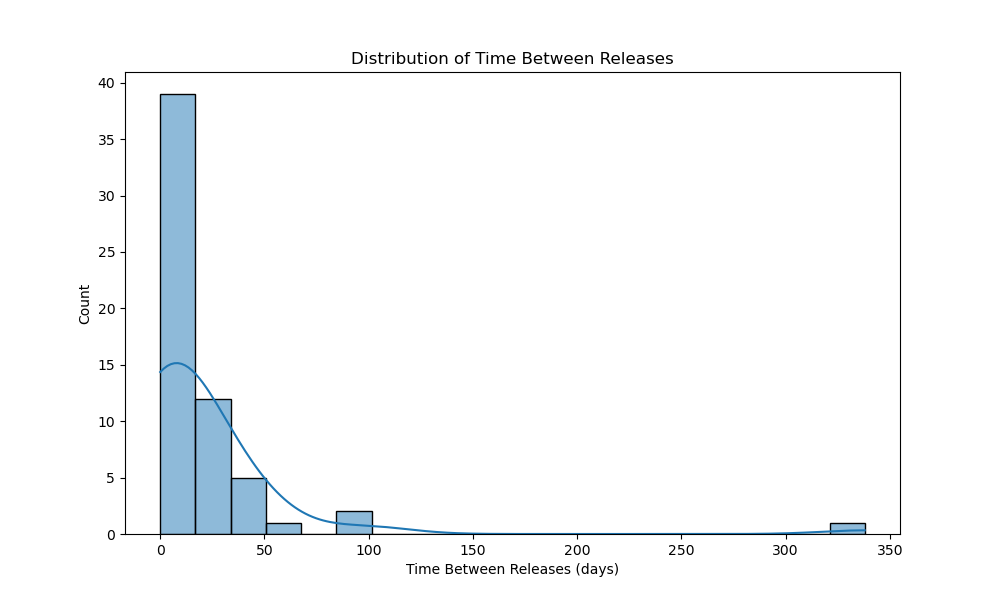
\includegraphics[width=0.9\textwidth]{images/time_between_releases_histogram.png} 
  \caption{Time between releases histogram}
  \label{fig:releases_frequency_histogram}
\end{figure}

\begin{figure}[h!] 
  \centering
  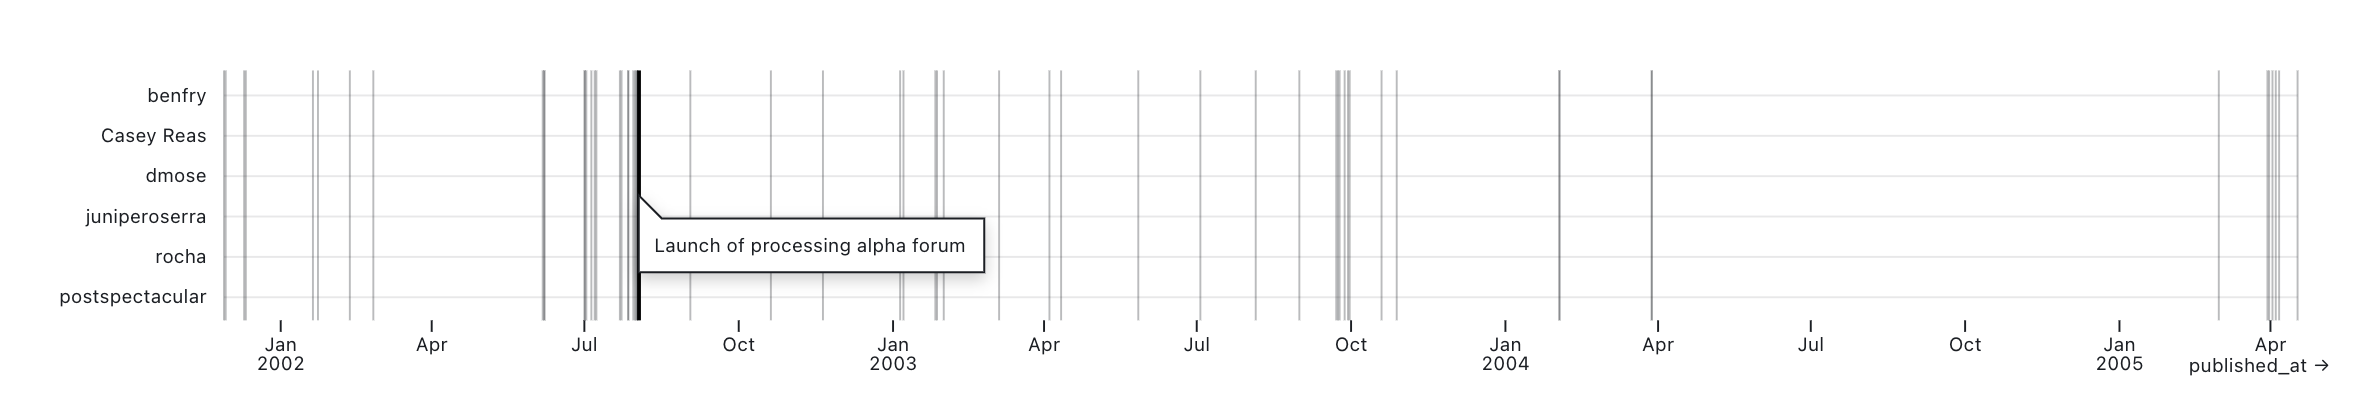
\includegraphics[width=0.9\textwidth]{images/releases-lines.png} 
  \caption{Time between releases}
  \label{fig:releases-lines}
\end{figure}

What makes Processing a particularly interesting case is that, contrary to what one might expect from Raymond's model, most contributions appear to be made by a centralized figure—Ben Fry, the project's main architect—rather than a broad community of external contributors. This effectively shifts the project's development model closer to a cathedral-like structure for core components, as reflected by Ben's direct control over major releases. 

Moreover, the project’s side-project nature is confirmed by revision comments such as one from 05/01/2003, which reads: "hopefully January 2003 will be a good month for p5, as I have a short bit of time to work on it [...] I hope to get a few revisions out this month so I can get back to my 'real' work." These comments illuminate that, for core contributors, Processing is not necessarily viewed as a full-time commitment.

The perception of Processing as a side project rather than a full-time commitment for its core contributors is corroborated through multiple channels. For example, a revision comment from May 1, 2003, highlights this sentiment, stating, ``hopefully January 2003 will be a good month for p5, as I have a short bit of time to work on it [...] I hope to get a few revisions out this month so I can get back to my `real' work.'' This observation is further substantiated by a 2021 study titled ``Graphic design in the post-digital age: a survey of practices fueled by creative coding,'' which notes that Processing began as a personal initiative and was largely developed during nights and weekends. The study further reveals that the project received indirect funding from MIT through Fry's graduate stipend, and from IDII through Reas's salary, again indicating its ancillary nature in the professional lives of its principal contributors~\parencite[396]{conradGraphicDesignPostdigital2021}.

It is worth noting that the logistics of releasing software were more complex in the early 2000s than they are today. As can be seen in Figure~\ref{fig:processing-cd} of a mini CD from October 2002 illustrates, distributing software was not as straightforward as pushing updates to a Git repository.

\begin{figure}[h!] 
  \centering
  
\includegraphics[width=0.9\textwidth]{images/processing-mini-cd.jpg} 
  \caption{MINI CDs CREATED FOR SPONSORS at the MEDIA LAB OPEN HOUSE october 2002}
  \label{fig:processing-cd}
\end{figure}

\subsubsection{Trends in Git Commits}

The \textit{Processing} project illuminates a crucial challenge often faced by open source communities: the dependency on key contributors. In the case of Processing, Ben Fry's central role over the past two decades raises concerns about the project's resilience and sustainability. His substantial contributions create a high-risk situation termed the "bus factor" \parencite{BusFactor2023}, which indicates how vulnerable a project becomes when overly reliant on a single or a small number of contributors. This vulnerability is not unique to Processing, as such dependency models are commonly observed across open source projects, often humorously discussed in popular culture \parencite{munroeDependency2020}.

The imbalanced contribution landscape is vividly illustrated in Figure~\ref{fig:alpha-commits}. During the period of the alpha forum, only six individuals contributed code to the repository. This stands in stark contrast to the activity on the forum, where over 1000 individuals were engaged in discussions and queries. The commits themselves were also sporadic and infrequent. As Casey aptly points out: ``I think one thing that’s important to clarify is that Ben Fry, my collaborator, is the primary software engineer of the project [...]'' \parencite[p. 330]{conradGraphicDesignPostdigital2021}.

\begin{figure}[h!] 
  \centering 
  \includesvg[pretex=\sffamily\fontsize{5.58pt}{8pt}\selectfont, width=1\textwidth, keepaspectratio]{images/processing-alpha-commits.svg}
  \caption{Commits up to and including the Processing alpha forum}
  \label{fig:alpha-commits}  
\end{figure}

This discrepancy between the number of code contributors and forum participants is indeed profound, as corroborated by the subsequent visualizations ~\ref{fig:top12-github} and comic anecdotes ~\ref{fig:dependency_comic}. The limited number of contributors to the codebase and the concentrated responsibility on a few individuals amplify the bus factor risk, an issue that warrants deeper investigation and consideration for the long-term health of the project.


\begin{figure}[h!] 
    \centering 
    \includesvg[pretex=\sffamily\fontsize{5.58pt}{8pt}\selectfont, width=1\textwidth, keepaspectratio]{images/figure-top12-github.svg}
    \caption{Top 12 source code contributors by number of commits}
    \label{fig:top12-github}  
  \end{figure}

\begin{figure}[h!] 
    \centering
    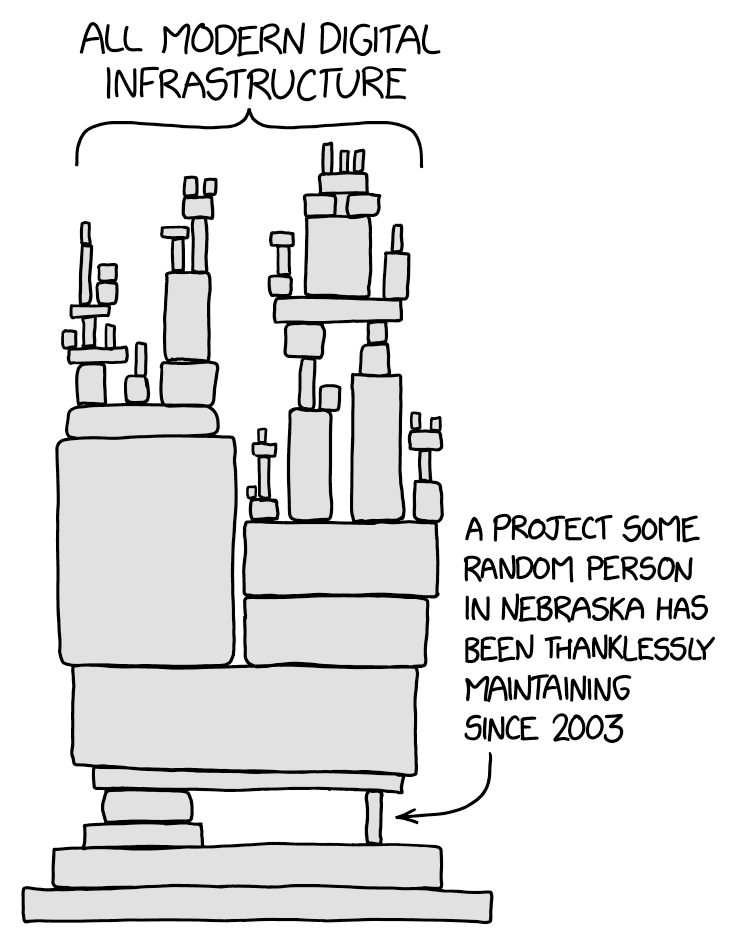
\includegraphics[width=0.5\textwidth]{dependency.png} 
    \caption{Dependency}
    \label{fig:dependency_comic}
    \small Source: \textit{XKCD}, \url{https://xkcd.com/2347/}, licensed under CC BY-NC 2.5.
\end{figure}

% \subsubsection{Patterns in Forum Contributions}

% Although Ben Fry remains the most active contributor in forum discussions, the activity distribution is more balanced compared to Git commits. This may be due to the broader range of topics discussed, including technical issues and bugs.
% A total of 1039 people posted on the forum in that time period. There were core people there that were actively participating as can be seen in the ~ref{processing-alpha-dot}

% Casey Reas “I would say that the period from around 2002 to 2006 was one when it felt almost like a unified international community created around the forum.” ([“Graphic design in the post-digital age: a survey of practices fueled by creative coding”, 2021, p. 331](zotero://select/library/items/GKA2GIS5)) ([pdf](zotero://open-pdf/library/items/QL4IRL3M?page=333&annotation=BRCSCF56))

% \begin{figure}[h!] 
%   \centering
%   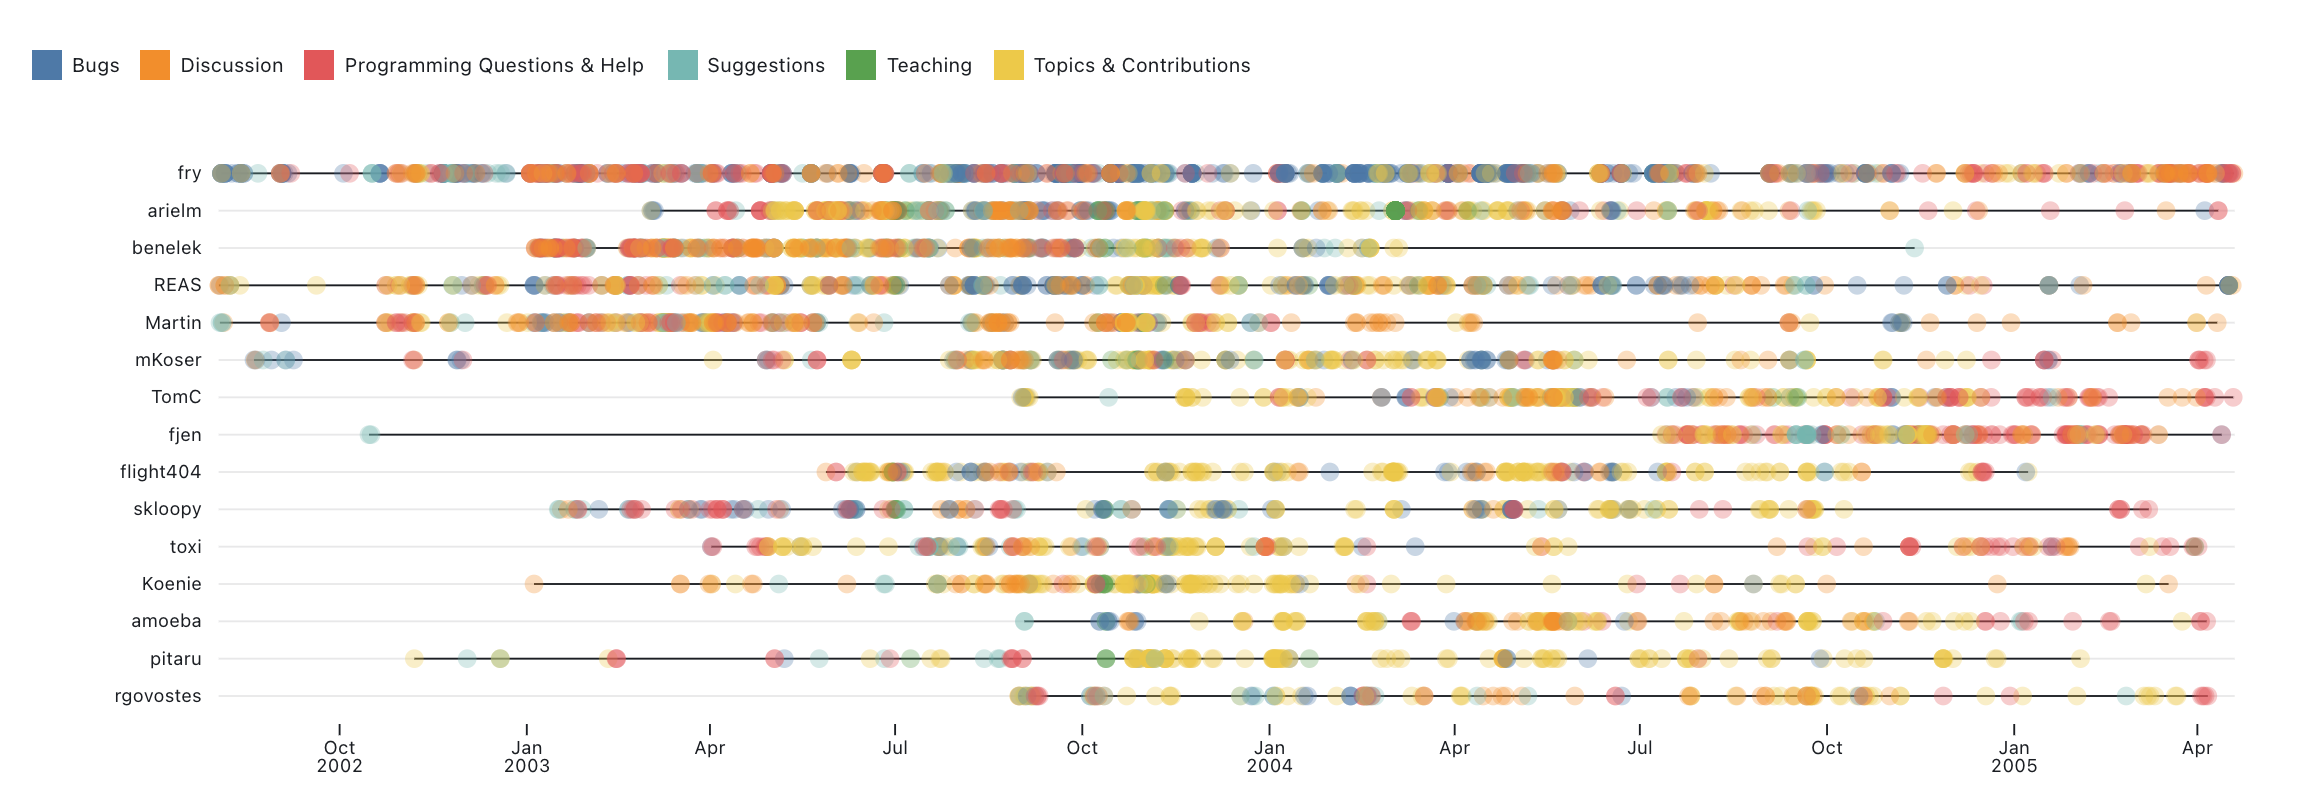
\includegraphics[width=0.9\textwidth]{images/alpha-forum-top15.png} 
%   \caption{Posting of 15 most active contributors on the alpha forum}
%   \label{fig:processing-alpha-dot}
% \end{figure}

% “"Given enough eyeballs, all bugs are shallow." I dub this: "Linus's Law."” ([Raymond, 1999, p. 29](zotero://select/library/items/87U5FDLI)) ([pdf](zotero://open-pdf/library/items/UZP875I7?page=7&annotation=89BX42PF))
% While this didn't translate well to the number of code contributors, we can see an incresed activity in the forum adjacent to releases suggesting that people contribute to at least finding bugs as seen in ~ref{figure:forum-git-activity}

\subsubsection{Patterns in Forum Contributions}

Ben Fry is the most active forum contributor, but the activity distribution is more balanced than in Git commits, possibly due to the diverse topics covered, including technical queries and bugs. A total of 1,039 individuals contributed to the forum discussions as shown in Figure~\ref{fig:processing-alpha-dot}.

Casey Reas suggests that from 2002 to 2006, the forum cultivated a "unified international community" \parencite[331]{conradGraphicDesignPostdigital2021}. 


% todo create a whole new document that is jsut this size
% Start a new page with a new size
\clearpage
% \pdfpagewidth=\diagramPaperWidth % New width for the following pages
% \pdfpageheight=\paperHeight % New height for the following pages

\begin{figure}[h!]
  \centering
  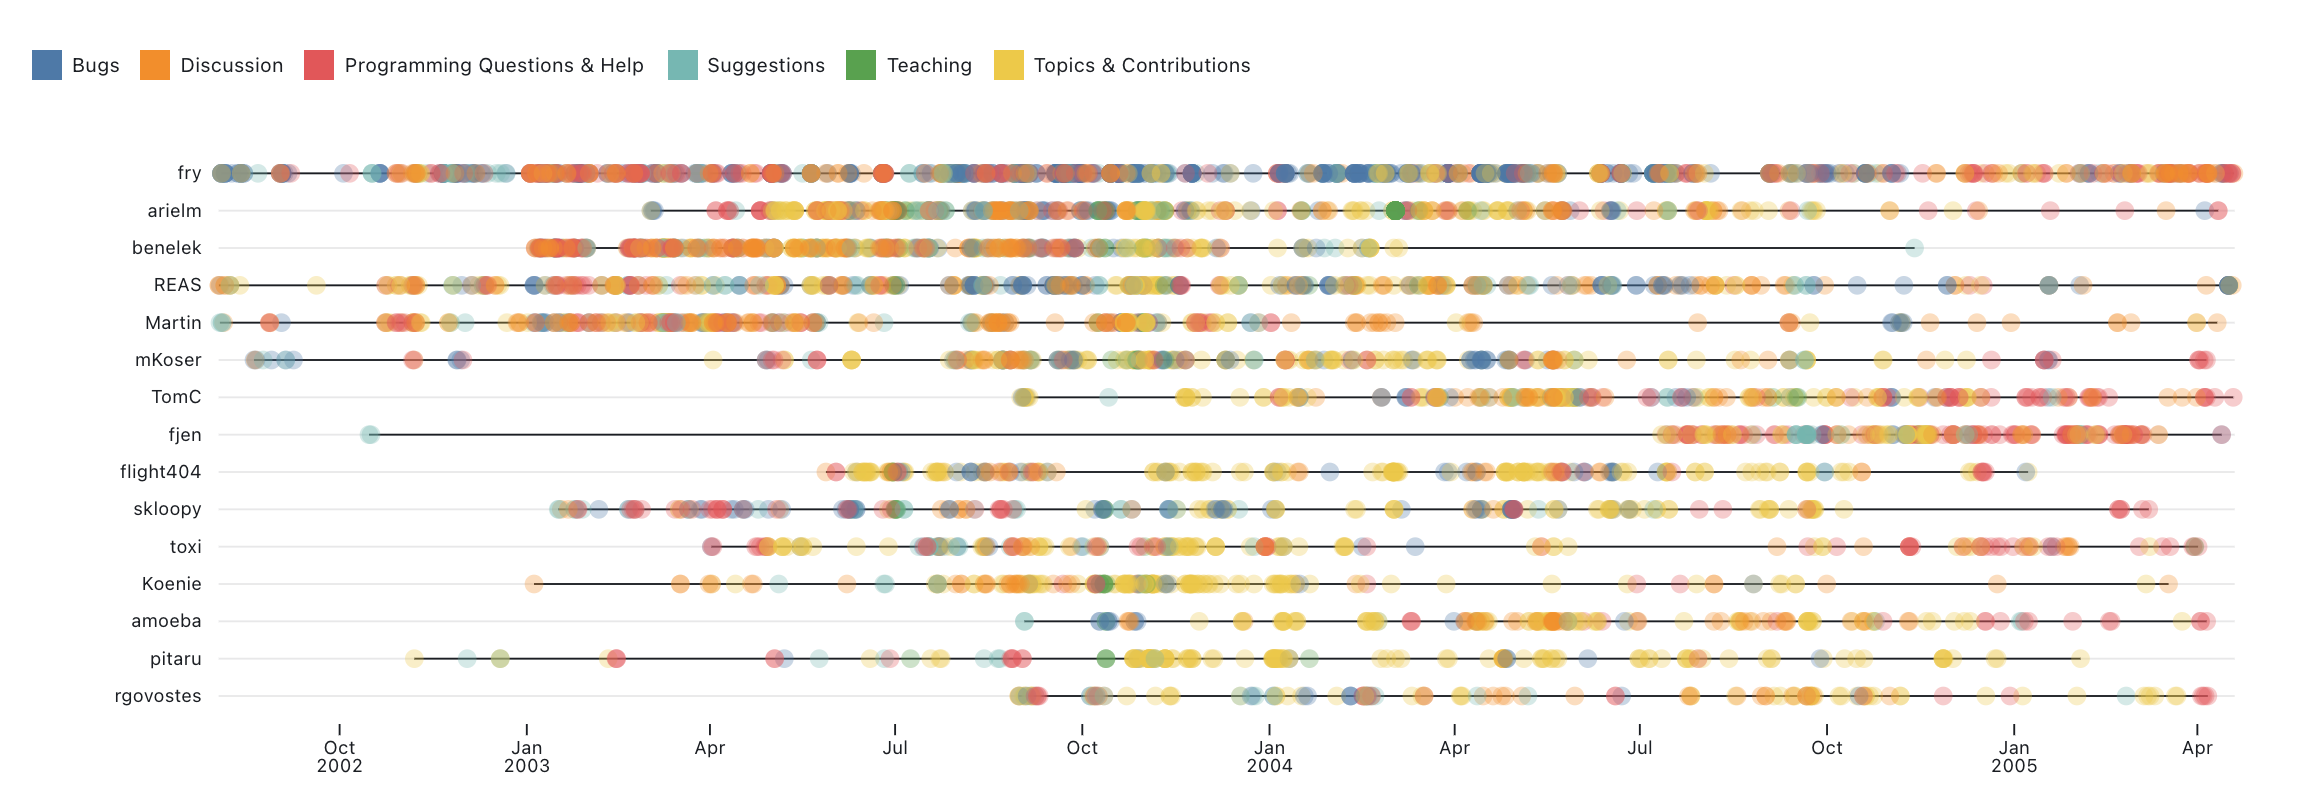
\includegraphics[width=1.0\textwidth]{images/alpha-forum-top15.png}
  \caption{Posting activity of the 15 most active contributors on the alpha forum.}
  \label{fig:processing-alpha-dot}
\end{figure}

% Revert to the original size
\clearpage

% \pdfpagewidth=\paperWidth % Width of A4 paper
% \pdfpageheight=\paperHeight % New height for the following pages
% \clearpage
% \restoregeometry


Linus's Law—"Given enough eyeballs, all bugs are shallow" \parencite[29]{raymondCathedralBazaar1999}—is somewhat evidenced by increased forum activity during release periods, suggesting community involvement in bug identification, as demonstrated in Figure~\ref{figure:forum-git-activity}.

\begin{figure}[!htbp] 
    \centering 
    %\includesvg[pretex=\sffamily\fontsize{5.58pt}{8pt}\selectfont, width=1\textwidth, keepaspectratio]{images/figure-forum-git-activity.png}
    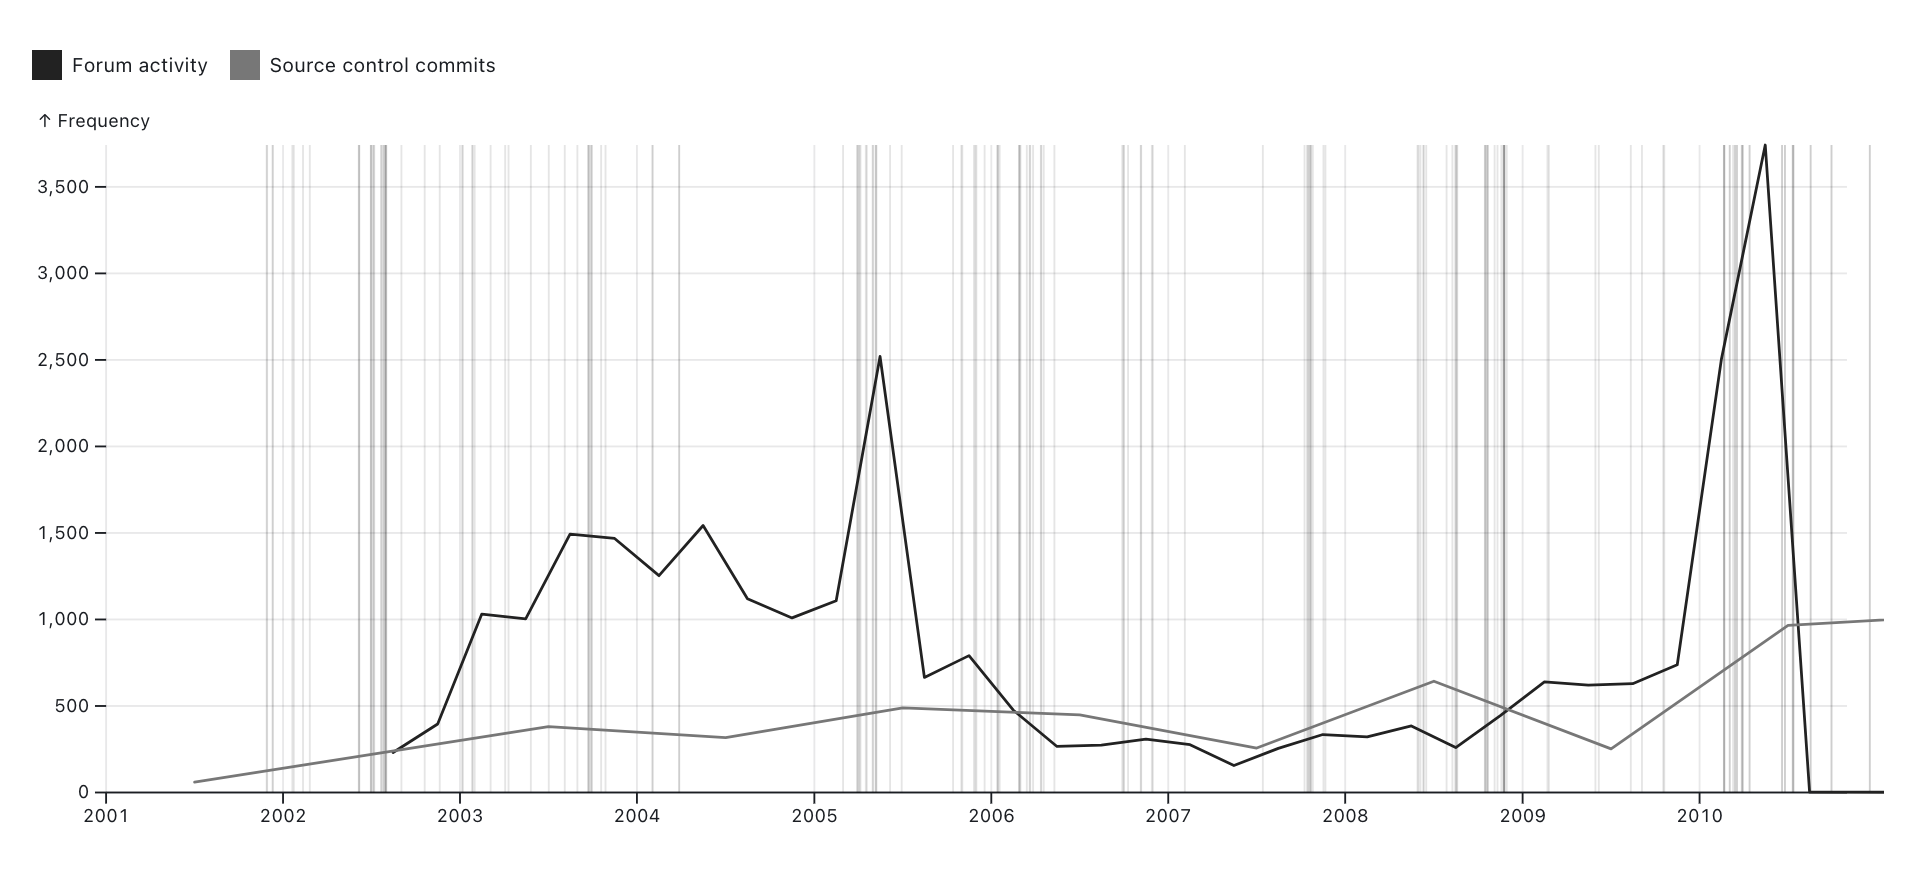
\includegraphics[width=1\textwidth]{images/figure-forum-git-activity.png} 

    \caption{Forum vs git activity vs releases (vertical lines)}
    \label{figure:forum-git-activity}  
  \end{figure}

Contrary to the initial assumption that primary contributors would predominantly be from the MIT ACG group, given the project's origins, a preliminary analysis suggests otherwise.

\begin{figure}[htbp]
  \centering
  
  % Row 1
  \begin{subfigure}[b]{0.24\textwidth}
      \includesvg[pretex=\sffamily\fontsize{5.58pt}{8pt}\selectfont, width=1\textwidth, keepaspectratio]{images/month1.svg}
      \caption{Month 1}
      \label{fig:month1}
  \end{subfigure}
  \hfill
  \begin{subfigure}[b]{0.24\textwidth}
    \includesvg[pretex=\sffamily\fontsize{5.58pt}{8pt}\selectfont, width=1\textwidth, keepaspectratio]{images/month2.svg}
      \caption{Month 2}
      \label{fig:month2}
  \end{subfigure}
  \hfill
  \begin{subfigure}[b]{0.24\textwidth}
    \includesvg[pretex=\sffamily\fontsize{5.58pt}{8pt}\selectfont, width=1\textwidth, keepaspectratio]{images/month3.svg}
      \caption{Month 3}
      \label{fig:month3}
  \end{subfigure}
  \hfill
  \begin{subfigure}[b]{0.24\textwidth}
    \includesvg[pretex=\sffamily\fontsize{5.58pt}{8pt}\selectfont, width=1\textwidth, keepaspectratio]{images/month4.svg}
      \caption{Month 4}
      \label{fig:month4}
  \end{subfigure}
  
  % Add space between rows
  \vspace{0.25cm}

  % Row 2
  \begin{subfigure}[b]{0.24\textwidth}
    \includesvg[pretex=\sffamily\fontsize{5.58pt}{8pt}\selectfont, width=1\textwidth, keepaspectratio]{images/month5.svg}
      \caption{Month 5}
      \label{fig:month5}
  \end{subfigure}
  \hfill
  \begin{subfigure}[b]{0.24\textwidth}
    \includesvg[pretex=\sffamily\fontsize{5.58pt}{8pt}\selectfont, width=1\textwidth, keepaspectratio]{images/month6.svg}
      \caption{Month 6}
      \label{fig:month6}
  \end{subfigure}
  \hfill
  \begin{subfigure}[b]{0.24\textwidth}
    \includesvg[pretex=\sffamily\fontsize{5.58pt}{8pt}\selectfont, width=1\textwidth, keepaspectratio]{images/month7.svg}
      \caption{Month 7}
      \label{fig:month 7}
  \end{subfigure}
  \hfill
  \begin{subfigure}[b]{0.24\textwidth}
    \includesvg[pretex=\sffamily\fontsize{5.58pt}{8pt}\selectfont, width=1\textwidth, keepaspectratio]{images/month8.svg}
      \caption{Month 8}
      \label{fig:month 8}
  \end{subfigure}

  % Add space between rows
  \vspace{0.25cm}

  % Row 3
  \begin{subfigure}[b]{0.24\textwidth}
    \includesvg[pretex=\sffamily\fontsize{5.58pt}{8pt}\selectfont, width=1\textwidth, keepaspectratio]{images/month9.svg}
      \caption{Month 9}
      \label{fig:month9}
  \end{subfigure}
  \hfill
  \begin{subfigure}[b]{0.24\textwidth}
    \includesvg[pretex=\sffamily\fontsize{5.58pt}{8pt}\selectfont, width=1\textwidth, keepaspectratio]{images/month10.svg}
      \caption{Month 10}
      \label{fig:month10}
  \end{subfigure}
  \hfill
  \begin{subfigure}[b]{0.24\textwidth}
    \includesvg[pretex=\sffamily\fontsize{5.58pt}{8pt}\selectfont, width=1\textwidth, keepaspectratio]{images/month11.svg}
      \caption{Month 11}
      \label{fig:month11}
  \end{subfigure}
  \hfill
  \begin{subfigure}[b]{0.24\textwidth}
    \includesvg[pretex=\sffamily\fontsize{5.58pt}{8pt}\selectfont, width=1\textwidth, keepaspectratio]{images/month12.svg}
      \caption{Month 12}
      \label{fig:month12}
  \end{subfigure}
  
  \caption{Monthly graphs}
  \label{fig:monthlyGraphs}
\end{figure}


\begin{figure}[h!] 
  \centering 
  \includesvg[pretex=\sffamily\fontsize{5.58pt}{8pt}\selectfont, width=1\textwidth, keepaspectratio]{images/year.svg}
  \caption{Year}
  \label{figure:year}  
\end{figure}


%\begin{figure}[h!] 
    \centering 
    \includesvg[pretex=\sffamily\fontsize{5.58pt}{8pt}\selectfont, width=1\textwidth, keepaspectratio]{images/figure-forum-posts.svg}
    \caption{Top 12 authors by number of posts (Aggregated alpha and beta forum)}
    \label{fig:forum-posts}  
  \end{figure}

%\begin{figure}[htbp] 
    \centering
    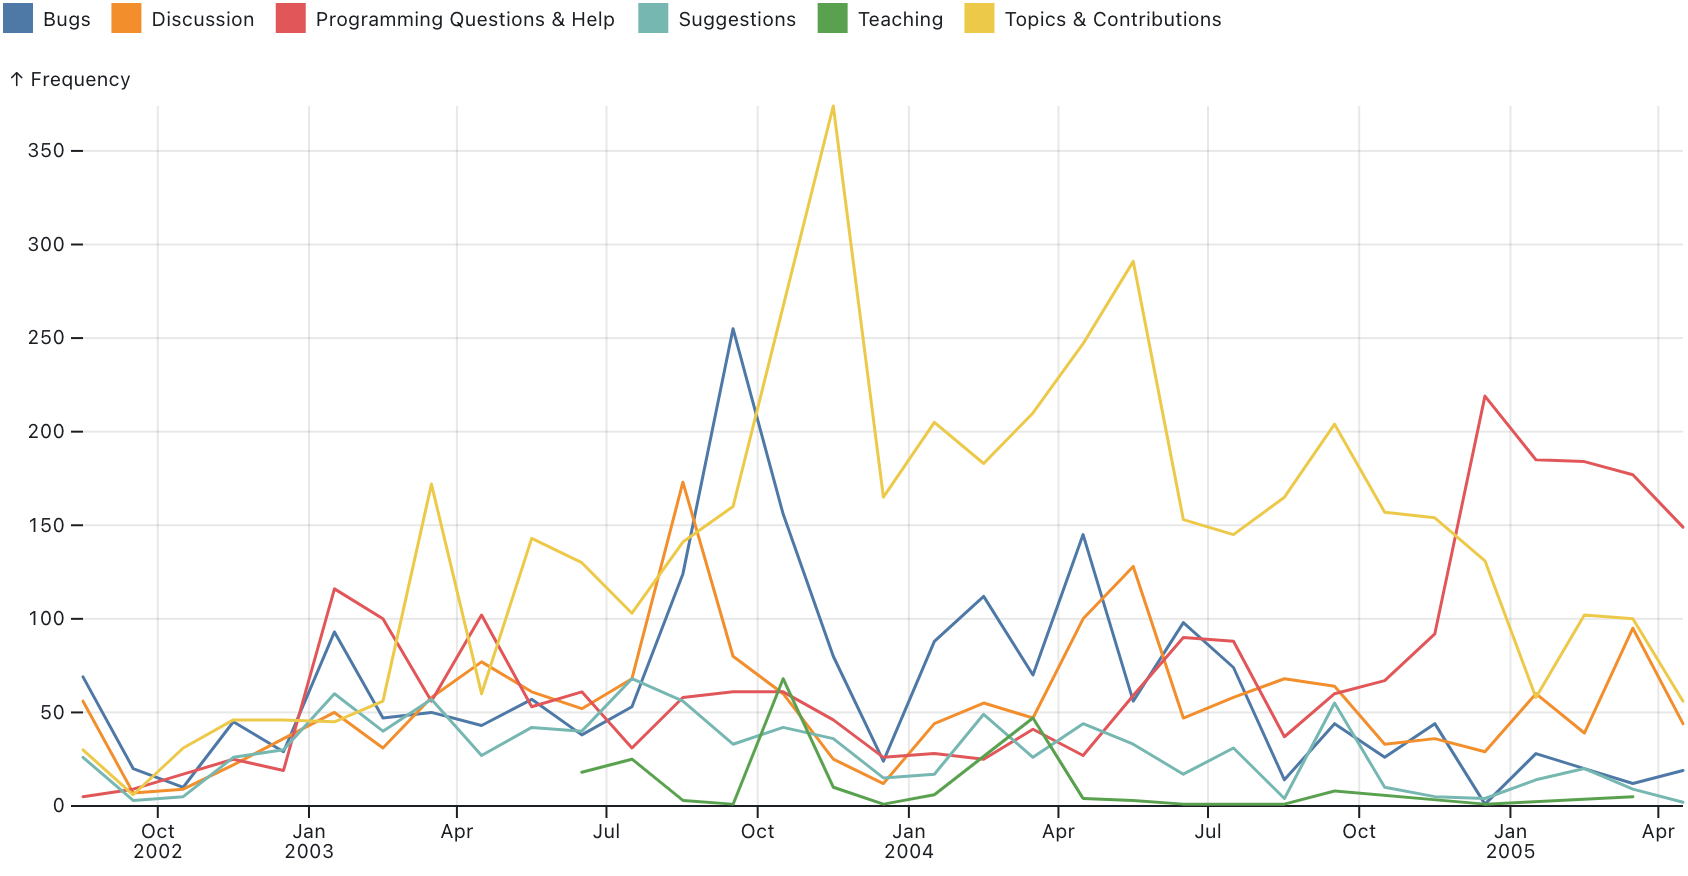
\includegraphics[width=1\textwidth]{alpha-forums-activity.png} 
    % \includesvg[pretex=\sffamily\fontsize{5.58pt}{8pt}\selectfont, width=0.6\textwidth]{images/alpha-forums-activity.svg}
    \caption{Forums activity}
    \label{fig:forum-activity}  
  \end{figure}

%\begin{figure}[h!] 
    \centering 
    \includesvg[pretex=\sffamily\fontsize{5.58pt}{8pt}\selectfont, width=1\textwidth, keepaspectratio]{images/figure-alltime-sourcecode-commits.svg}
    \caption{Top 25 source code contributors by number of commits}
    \label{fig:alltime-sourcecode-commits}  
  \end{figure}

%\begin{figure}[htbp] 
    \centering
    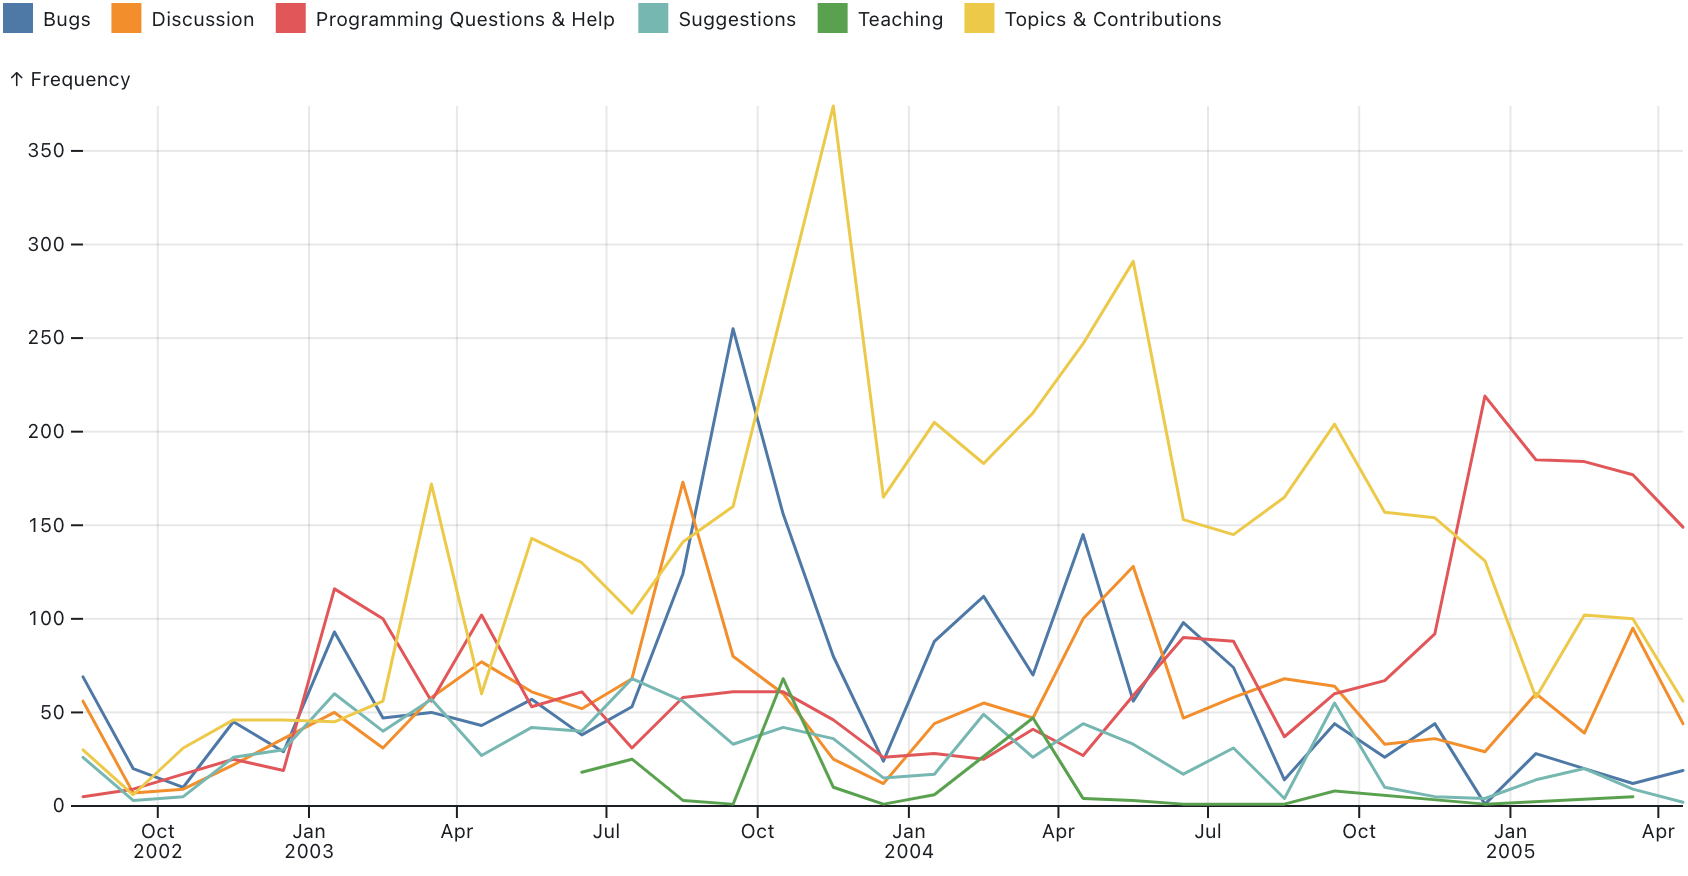
\includegraphics[width=1\textwidth]{alpha-forums-activity.png} 
    % \includesvg[pretex=\sffamily\fontsize{5.58pt}{8pt}\selectfont, width=0.6\textwidth]{images/alpha-forums-activity.svg}
    \caption{Forums activity}
    \label{fig:forum-activity}  
  \end{figure}

% \subsubsection{Synthesized Data Analysis: Git Commits, Releases, and Forum Activity}

\newpage
\subsubsection{Alpha Forum Patterns in Forum Contributions (to remove)}
There were 11,926 posts across 2,626 topics from 02/08/2002, 15:29 to the 19/04/2005, 09:55 across 1039 authors in the forum.

The alpha forum was a YaBB (Yet another Bulletin Board), it was seperated into forums which conained boards which contained topics which contained posts.

\begin{figure}
    \centering 
    \includesvg[pretex=\sffamily\fontsize{5.58pt}{8pt}\selectfont, width=1\textwidth, keepaspectratio]{images/alpha-forums-by-posts.svg}
    \caption{Topics by post number}
    \label{fig:forums}  
  \end{figure}

% todo add
% \subsection{Qualitative Insights}
% \subsubsection{Themes from the Forum}
% \subsubsection{Interview Highlights and Key Takeaways}

% \section{Discussion}

% \subsection{Integrating Quantitative and Qualitative Findings}
% \subsection{Implications for the Open Source Community}
% \subsection{The Unique Case of Processing and Creative Coding}
% \subsection{Limitations of the Study}

% \section{Conclusion and Recommendations}

% \subsection{Recap of Key Findings}
% \subsection{Practical Implications for Open Source Projects}
% \subsection{Recommendations for Future Research}
